%
% abbildungen.tex -- Lineare Abbildungen
%
% (c) 2018 Prof Dr Andreas Müller, Hochschule Rapperswil
%
\section{Lineare Abbildungen%
\label{skript:section:lineare abbildungen}}
Wie im vorangegangenen Abschnitt verwenden wir im folgenden eine Basis
$\mathcal{B}=\{\vec{b}_1,\dots,\vec{b}_n\}$, die Vektoren $\vec{v}_i$
sind linear unabhängig, und jeder Vektor lässt sich als Linearkombination
dieser Basisvektoren schreiben.

%
% Affine Abbildungen
%
\subsection{Affine und lineare Abbildungen}
Wenn man von einem Problem einen Plan machen, dann darf die Perspektive
keine Rolle spielen.
Der Plan darf keine für das Problem wesentlichen Eigenschaften stören.
Auf ein mathematisches Problem übertragen müssen wir in der Lage sein,
Abbildungen auf das Problem anzuwenden, welche helfen können, das
Problem zu lösen.
Diese Abbildungen dürfen die wesentlichen Eigenschaften der untersuchten
Objekte nicht verändern.

Die dem Abschnitt~\ref{skript:koordinaten} vorangestellten Axiome
sprechen von Geraden, Ebenen und Parallelen als den primären geometrischen
Objekten.
Zulässige Abbildungen dürfen also Ebenen und Geraden nicht zerstören.
Wenn aber Geraden auf Geraden abgebildet werden, dann werden Geraden,
die sich nicht schneiden, auf Geraden abgebildet, die sich nicht schneiden,
Parallelität ist also automatisch erhalten.

\begin{definition}
Eine Abbildung, die Ebene, Geraden und Parallelität erhält,
heisst {\em affine Abbildung}
\end{definition}
\index{affine Abbildung}

Aus den Axiomen haben wir die algebraischen Eigenschaften von Ortsvektoren
konstruiert.
Affine Abbildungen müssen also verträglich sein mit den algebraischen
Operationen.
Um die Geometrie mit Vektoren auszudrücken, mussten wir ausserdem
einen ausgezeichneten Punkt $O$ haben.
Dieser muss natürlich unter Abbildungen, die uns interessieren
ebenfalls erhalten bleiben.
Eine affine Abbildung $\varphi$ muss also folgende Regeln erfüllen:
\begin{align*}
\varphi(O)&=O
\\
\varphi(\lambda\vec{p})&=\lambda\varphi(\vec{p})
\\
\varphi(\vec{u}+\vec{v})&=\varphi(\vec{u}) + \varphi(\vec{v})
\end{align*}

\begin{definition}
Eine Abbildung $\varphi\colon \mathbb R^n \to \mathbb R^m$ mit den
Eigenschaften
\begin{align*}
\varphi(\lambda\vec{p})&=\lambda\varphi(\vec{p})
&&\text{und}&
\varphi(\vec{u}+\vec{v})&=\varphi(\vec{u}) + \varphi(\vec{v})
\end{align*}
heisst {\em linear}.
\end{definition}

%
% Beschreibung linearer Abbildungen mit Matrizen
%
\subsection{Beschreibung linearer Abbildungen mit Matrizen}
Wir wollen jetzt lineare Abbildungen der Ebene und des dreidimensionalen
Raumes mit Hilfe einer Basis genauer beschreiben.
Sei also eine Basis $\mathcal{B}=\{\vec{b}_1,\dots,\vec{b}_n\}$ 
gegeben und eine lineare Abbildung $\varphi$.

\subsubsection{Matrix einer linearen Abbildung}
Jeder beliebige Vektor $\vec{x}$ kann als Linearkombination
\[
\vec{x}
=
x_1\vec{b}_1
+\dots+
x_n\vec{b}_n
\]
der Vektoren $\vec{b}_i$ geschrieben werden.
Der Bildvektor $\varphi(\vec{x})$ kann mit den Linearitätseigenschaften
vereinfacht werden:
\[
\varphi(\vec{x})
=
\varphi(
x_1\vec{b}_1
+\dots+
x_n\vec{b}_n
)
=
x_1\varphi(\vec{b}_1)
+\dots+
x_n\varphi(\vec{b}_n).
\]
Die lineare Abbildung ist also vollständig durch die Bilder der Basisvektoren
$\varphi(\vec{b}_i)$ festgelegt.

In der Basis werden die Vektoren $\vec{b}_i$ durch die Standardbasisvektoren
\[
\vec{e}_1 = \begin{pmatrix}1\\0\\\vdots\\0\end{pmatrix},\quad
\vec{e}_2 = \begin{pmatrix}0\\1\\\vdots\\0\end{pmatrix},
\quad\dots,\quad
\vec{e}_n = \begin{pmatrix}0\\0\\\vdots\\1\end{pmatrix}
\]
dargestellt.
Auch die Bildvektoren können in der Basis $\mathcal{B}$ ausgedrückt werden,
wir schreiben die Bilder als Spaltenvektoren
\[
\vec{a}_i
=
\varphi(\vec{b}_i)
=
\begin{pmatrix}
a_{1i}\\a_{2i}\\\vdots\\a_{ni}
\end{pmatrix}.
\]
Der Bildvektor $\varphi(\vec{x})$ ist daher die Linearkombination
\[
\varphi(\vec{x})
=
x_1
\begin{pmatrix}
a_{11}\\a_{21}\\\vdots\\a_{n1}
\end{pmatrix}
+
x_2
\begin{pmatrix}
a_{12}\\a_{22}\\\vdots\\a_{n2}
\end{pmatrix}
+
\dots
+
x_n
\begin{pmatrix}
a_{1n}\\a_{2n}\\\vdots\\a_{nn}
\end{pmatrix}
=
\begin{pmatrix}
a_{11}&a_{12}&\dots &a_{1n}\\
a_{21}&a_{22}&\dots &a_{2n}\\
\vdots&\vdots&\ddots&\vdots\\
a_{21}&a_{22}&\dots &a_{2n}
\end{pmatrix}
\begin{pmatrix}
x_1\\x_2\\\vdots\\x_n
\end{pmatrix}
\]
Die Spalten der Matrix $A$ sind die Koordinatenvektoren der Bilder
$\varphi(\vec{b}_i)$.
Wir fassen diese Resultate wie folgt zusammen.

\begin{satz}
\label{satz:affin:bilderderstandardbasisvektoren}
Eine lineare Abbildung wird durch die Matrix $A$ vollständig beschrieben,
die Spalten enthalten die Bilder der Standardbasisvektoren.
\end{satz}

\subsubsection{Beispiel: Vertauschung der Achsen}
Wir suchen die Matrix der linearen Abbildung, die die beiden Achsrichtungen
$\vec{e}_1$ und $\vec{e}_2$ verauscht.
In den Spalten von $A$ stehen die Bilder der Standardbasisvektoren,
daher muss in der ersten Spalte das Bild von $\vec{e}_1$ stehen, also
der Vektor $\vec{e}_2$.
In der zweiten Spalte muss dagegen $\vec{e}_1$ stehen.
Die gesuchte Matrix ist daher
\[
A=\begin{pmatrix}0&1\\1&0\end{pmatrix}.
\]

\subsubsection{Beispiel: Matrix einer Spiegelung}
\begin{figure}
\centering
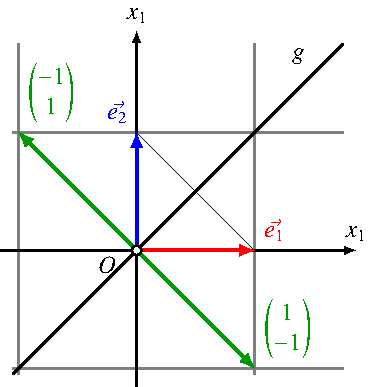
\includegraphics{3/images/spiegelung.pdf}
\caption{Die Spiegelung an der Geraden $g$ bildet den Vektor
$\vec{e}_1$ auf $\vec{e}_2$ ab und umgekehrt.
\label{skript:affin:spiegelung}}
\end{figure}
Wir suchen die Matrix einer Spiegelung der Ebene an der Geraden durch
die Punkte $O$ und $(2,2)$.
Nach Satz~\label{satz:affin:bilderderstandardbasisvektoren} müssen wir 
die Bilder der Standardbasisvektoren bestimmen.
Aus Abbildung~\ref{skript:affin:spiegelung} kann man ablesen, dass die
Spiegelung den Vektor $\vec{e}_1$ auf $\vec{e}_2$ abbildet und umgekehrt.
Daraus kann man jetzt die Matrix $S$ der Spiegelung zusammensetzen,
sie enthält die Bilder der Standardbasisvektoren:
\[
\vec{e}_1\leftrightarrow\vec{e}_2
\qquad\Leftrightarrow\qquad
\begin{pmatrix}1\\0\end{pmatrix}
\leftrightarrow
\begin{pmatrix}0\\1\end{pmatrix}
\qquad\Leftrightarrow\qquad
S
=
\begin{pmatrix}0&1\\1&0\end{pmatrix}.
\]
Wir kontrollieren dieses Resultate, indem wir berechnen wie ein Vektor
auf der Geraden und senkrecht dazu abgebildet wird:
\begin{align*}
S
\begin{pmatrix}1\\1\end{pmatrix}
&=
\begin{pmatrix}0&1\\1&0\end{pmatrix}
\begin{pmatrix}1\\1\end{pmatrix}
=
\begin{pmatrix}1\\1\end{pmatrix}
\\
S
\begin{pmatrix}1\\-1\end{pmatrix}
&=
\begin{pmatrix}0&1\\1&0\end{pmatrix}
\begin{pmatrix}1\\-1\end{pmatrix}
=
\begin{pmatrix}-1\\1\end{pmatrix}
=
-
\begin{pmatrix}1\\-1\end{pmatrix}.
\end{align*}
Der Vektor in der zweiten Zeile steht senkrecht auf der Geraden $g$ 
und wird durch die Spiegelung mit $-1$ multipliziert.

Natürlich ist dies genau die gleiche Matrix wie im vorangegangenen
Beispiel, denn die Spiegelung vertauscht natürlich die beiden
Basisvektoren.

\subsubsection{Beispiel: Matrix einer Drehung}
\begin{figure}
\centering
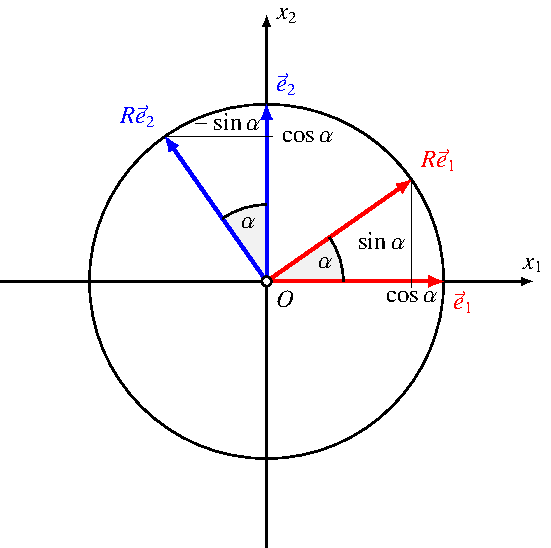
\includegraphics{3/images/drehung.pdf}
\caption{Drehung der Ebene um den Winkel $\alpha$.
Die Drehmatrix $R$ besteht aus den Bildern der Standardbasisvektoren.
\label{skript:affin:drehung}}
\end{figure}
Gesucht ist die Matrix $R$ einer Drehung um den Winkel $\alpha$.
Aus Abbildung~\ref{skript:affin:drehung} liest man die Bilder der
Standardbasisvektoren ab:
\[
R\colon \vec{e}_1 \mapsto \begin{pmatrix}\cos\alpha\\\sin\alpha\end{pmatrix},
\qquad
R\colon \vec{e}_2 \mapsto \begin{pmatrix}-\sin\alpha\\\cos\alpha\end{pmatrix}.
\]
Daraus kann man die Drehmatrix
\[
R=\begin{pmatrix}\cos\alpha&-\sin\alpha\\\sin\alpha&\cos\alpha\end{pmatrix}
\]
zusammensetzen.

%
% Komposition linearer Abbildungen
%
\subsection{Zusammensetzung linearer Abbildungen}
Was für eine Matrix erhält man, wenn man zwei lineare Abbildungen,
je beschrieben durch Matrizen $A$ und $B$ nacheinander ausführt?
Diese Situation kann schematisch dargestellt werden durch das Diagramm
\begin{equation}
\definecolor{darkgreen}{rgb}{0,0.6,0}
\xymatrix{
{\color{red}\mathbb R^n } \ar[r]^{A} \ar@/_20pt/[rr]_{C}
&{\color{darkgreen}\mathbb R^m} \ar[r]^{B}
&{{\color{blue}\mathbb R^l}.}
}
\label{skript:affin:komposition:diagramm}
\end{equation}
Um die Matrix dieser Zusammensetzung zu finden muss man herausfinden,
auf welche Vektoren die Standardbasisvektoren abgebildet werden.
Die erste Abbildung mit Matrix $A$ bildet $\color{red}\vec{e}_i$,
$i=1,\dots,n$, auf die $i$-te Spalte von $A$ ab, die wir mit
\begin{equation}
\definecolor{darkgreen}{rgb}{0,0.6,0}
{\color{darkgreen}\vec{a}_i}
=\begin{pmatrix}
{\color{darkgreen}a_{1i}}\\\vdots\\{\color{darkgreen}a_{mi}}
\end{pmatrix}
=
{ \color{darkgreen} a_{1i} \vec{e}_1}
+\dots +
{ \color{darkgreen} a_{mi} \vec{e}_m}
\label{skript:affin:komposition:a}
\end{equation}
bezeichnen.
Die zweite Abbildung bildet die Standardbasisvektoren in
$\definecolor{darkgreen}{rgb}{0,0.6,0}
\color{darkgreen}\mathbb R^m$ auf die Spalten
von $B$ ab.
Die Zusammensetzung \eqref{skript:affin:komposition:diagramm}
bildet den Vektor 
$\definecolor{darkgreen}{rgb}{0,0.6,0}
\color{darkgreen}
\vec{a}_i$ in \eqref{skript:affin:komposition:a} 
ab auf 
{%
\definecolor{darkgreen}{rgb}{0,0.6,0}%
\begin{align*}
B{\color{darkgreen}\vec{a_i}}
&=
{\color{blue}\vec{b}_1} {\color{darkgreen}a_{1i}}+\dots
+{\color{blue}\vec{b}_m}{\color{darkgreen}a_{mi}}
=
{\color{blue}
\begin{pmatrix}b_{11}\\\vdots\\b_{l1}\end{pmatrix}} {\color{darkgreen}a_{1i}}
+\dots+
{\color{blue}
\begin{pmatrix}b_{1m}\\\vdots\\b_{lm}\end{pmatrix}} {\color{darkgreen}a_{mi}}
=
{\color{blue}
\begin{pmatrix}
\color{black}
{\color{blue}b_{11}}{\color{darkgreen}a_{1i}}+\dots+{\color{blue}b_{1m}}{\color{darkgreen}a_{mi}}\\
\color{black} \vdots\\
\color{black}
{\color{blue}b_{l1}}{\color{darkgreen}a_{1i}}+\dots+{\color{blue}b_{lm}}{\color{darkgreen}a_{mi}}\\
\end{pmatrix}
}.
\end{align*}}
Dies ist aber auch die $i$-te Spalte der Matrix $C$, bestehend aus den
Komponenten $c_{1i}$ bis $c_{li}$.
Man liest ab
{
\definecolor{darkgreen}{rgb}{0,0.6,0}
\begin{align*}
c_{ji}
&=
{\color{darkgreen}b_{j1}}{\color{blue}a_{1i}} + \dots
	+ {\color{darkgreen}b_{jm}}{\color{blue}a_{mi}}
\\
\begin{pmatrix}
\qquad&\quad&\qquad\\
\qquad&c_{ji}&\qquad\\
\qquad&\quad&\qquad\\
\end{pmatrix}
&=
\begin{pmatrix}
&\dots&\\
\color{darkgreen}b_{j1}&\color{darkgreen}\dots&\color{darkgreen}b_{jm}\\
&\dots&
\end{pmatrix}
\begin{pmatrix}
&\qquad&\color{blue}a_{1i}&\qquad&\\
&\vdots&\color{blue}\vdots&\vdots&\\
&     &\color{blue}a_{mi}&&
\end{pmatrix}
\end{align*}
}
Dies ist genau die Definition des Matrizen-Produktes aus
Abschnitt~\label{skript:subsection:matrizen}.

\begin{satz}
Die Matrix $C$ der Abbildung zusmmengesetzt aus der Abbildung
mit Matrix $A$ gefolgt von der Abbildung mit Matrix $B$ ist
$C=BA$.
\end{satz}

Man beachte die scheinbar `verkehrte' Reihenfolge der Faktoren.
Man erinnere sich aber daran, dass die die Vektoren, auf die die Matrizen
wirken, rechts von der Matrix hingeschrieben werden.
Die Wirkung der Matrix $C$ auf einen Vektor $v$ wird $Cv$ geschrieben.
Dies soll das gleiche sein, wie wenn zuerst $A$ wirkt, was den Bildvektor
$Av$ ergibt, und auf diesen Vektor wirkt jetzt $B$, geschrieben $B(Av)=BAv$.

%
% Basiswechsel
%
\subsection{Basiswechsel}
Eine lineare Abbildung wird in einer Basis $\color{red}\mathcal{B}$ durch
eine Matrix $\color{red}A$ beschrieben, in den Spalten stehen die Bilder
der Standardbasisvektoren.
Sowohl die Standardbasisvektoren wie auch die Komponenten in den
Spalten sind von der Basis abhängig, die Abbildungsmatrix $\color{red}A$
ist also ebenfalls basisabhängig.
Damit stellt sich die Frage, wie sich die Matrix ändert, wenn
man die Basis wechselt.

Wir möchten jetzt eine neue Basis $\color{blue}\mathcal{C}$ verwenden, die
Basistransformationsmatrix $T$ sei gegeben.
Die Matrix $T$ rechnet die Koordinaten eines Vektors in der Basis
$\color{red}\mathcal{B}$ um in Koordinaten in der Basis
$\color{blue}\mathcal{C}$.
Um das Bild eines Vektors $\vec{u}$ in der Basis $\color{blue}\mathcal{C}$ 
zu berechnen, muss man ihn erst in $\color{red}\mathcal{B}$ umrechnen, was
mit der inversen Matrix $T^{-1}$ geschehen kann.
Dann erst kann man $A$ anwenden, erhält dann aber einen Vektor
in der Basis $\color{red}\mathcal{B}$, man muss ihn also erst wieder
mit $T$ in die Basis $\color{blue}\mathcal{C}$ umrechnen.
Alles zusammen ist in der Basis $\mathcal{C}$ der Bildvektor 
$T{\color{red}A}T^{-1}u$.
Wir fassen das Resultat zusammen im folgenden Satz.

\begin{satz}
\label{skript:affin:basiswechsel:satz}
Sei $T$ die Transformationsmatrix, die Koordinaten von der Basis
$\color{red}\mathcal{B}$ in die Basis $\color{blue}\mathcal{C}$ umrechnet.
Die lineare Abbildung, die in der Basis $\color{red}\mathcal{B}$ durch die
Matrix $A$ beschrieben wird, wird in der Basis $\color{blue}\mathcal{C}$ durch
die Matrix
\[
{\color{blue}A'}=T{\color{red}A}T^{-1}
\]
beschrieben.
\end{satz}

Diese Situation kann auch im folgenden Diagramm
\begin{center}
\begin{tikzpicture}[>=latex,thick]
\fill[color=white] (-7.5,-1) rectangle (7.5,1);
\fill[color=red!10]  (-7.3,0.3) rectangle (0,1.7);
\fill[color=red!20]  (-1.7, 0.3) rectangle (1.7, 1.7);
\fill[color=blue!10]  (-7.3,-0.3) rectangle (0,-1.7);
\fill[color=blue!20] (-1.7,-0.3) rectangle (1.7,-1.7);
\node[color=blue] at (-1,-1) {$\mathbb R^n$};
\node[color=blue] at ( 1,-1) {$\mathbb R^n$};
\node[color=red] at (-1, 1) {$\mathbb R^n$};
\node[color=red] at ( 1, 1) {$\mathbb R^n$};
\node at (-5, 1) {Basis ${\color{red}\mathcal{B}}=\{\vec{b}_1,\dots,\vec{b}_n\}$:};
\node at (-5,-1) {Basis ${\color{red}\mathcal{C}}=\{\vec{c}_1,\dots,\vec{c}_n\}$:};
\draw[->,color=red] (-0.7,1)--(0.7,1);
\node[color=red] at (0,1) [above] {$A$};
\draw[->,color=blue] (-0.7,-1)--(0.7,-1);
\node[color=blue] at (0,-1) [above] {$A'$};
\draw[->] (-1,0.7)--(-1,-0.7);
\draw[->] ( 1,0.7)--( 1,-0.7);
\node at ( 1,0) [right] {$T$};
\node at (-1,0) [right] {$T$};
\draw[<-] (-1.3, 0.8) arc (150:210:1.6);
\node at (-1.5,0) [left] {$T^{-1}$};
\end{tikzpicture}
\end{center}
illustriert werden.
Die Abbildung $\color{blue}A'$ führt vom Vektorraum unten links zum
Vektorraum unten rechts.
Dieser Weg ist gleichbedeutend mit dem Umweg über die beiden Vektorräume
in der oberen Zeile.
Um von unten links nach oben links zu kommen, muss man die
Transformationsmatrix $T^{-1}$ verwenden.
Zusammengesetzt wird der Umweg durch $T{\color{red}A}T^{-1}$ beschrieben,
woraus wieder die Aussage des Satzes folgt.

\begin{beispiel}
In einem früheren Beispiel haben wir die Spiegelung an der $45^\circ$-Geraden
mit Hilfe der Matrix 
\[
S=\begin{pmatrix}0&1\\1&0\end{pmatrix}
\]
beschrieben.
Jetzt möchten wir ein Koordinatensystem verwenden, welches gegenüber
dem ursprünglichen um $45^\circ$ verdreht ist.
Wir möchten also die Basisvektoren
\[
\vec{c}_1 = \frac{1}{\sqrt{2}} \begin{pmatrix}1\\1\end{pmatrix}
\qquad\text{und}\qquad
\vec{c}_2 = \frac{1}{\sqrt{2}} \begin{pmatrix}-1\\1\end{pmatrix}
\]
verwenden und müssen daher die Transformationsmatrix $T$ für den
Basiswechsel vonder Standardbasis in die neue Basis
$\mathcal{C}=\{\vec{c}_1,\vec{c}_2\}$ ermitteln.
Wir verwenden zur Bestimmung von $T$ das
Tableau~\eqref{skript:affin:basistransformation-tableau}, also
\[
\begin{tabular}{|>{$}c<{$}>{$}c<{$}|>{$}c<{$}>{$}c<{$}|}
\hline
\frac1{\sqrt{2}}&-\frac1{\sqrt{2}}&1&0\\
\frac1{\sqrt{2}}&\frac1{\sqrt{2}}&0&1\\
\hline
\end{tabular}
\quad
\rightarrow
\quad
\begin{tabular}{|>{$}c<{$}>{$}c<{$}|>{$}c<{$}>{$}c<{$}|}
\hline
1&0&\frac1{\sqrt{2}}&\frac1{\sqrt{2}}\\
0&1&-\frac1{\sqrt{2}}&\frac1{\sqrt{2}}\\
\hline
\end{tabular}
\]
die Transformationsmatrix ist damit
\[
T
=
\frac1{\sqrt{2}}\begin{pmatrix}
1&1\\
-1&1
\end{pmatrix}
\quad\text{und}\quad
T^{-1}
=
\frac1{\sqrt{2}}\begin{pmatrix}
1&-1\\
1&1
\end{pmatrix}.
\]
Damit können wir jetzt die Abbildungsmatrix im neuen Koordinatensystem
berechnen:
\[
S'
=
TST^{-1}
=
\frac1{\sqrt{2}}\begin{pmatrix}
1&1\\
-1&1
\end{pmatrix}
\begin{pmatrix}
0&1\\1&0
\end{pmatrix}
\frac1{\sqrt{2}}\begin{pmatrix}
1&-1\\
1&1
\end{pmatrix}
=
\frac12
\begin{pmatrix}
1&1\\1&-1
\end{pmatrix}
\begin{pmatrix}
1&-1\\1&1
\end{pmatrix}
=
\frac12
\begin{pmatrix}
2&0\\0&-2
\end{pmatrix}
=
\begin{pmatrix}
1&0\\0&-1
\end{pmatrix}
\]
Im neuen Koordinatensystem wird die Abbildung durch die Matrix $S'$
beschrieben.
Diese Matrix besagt, dass der erste Basisvektor nicht verändert wird,
während der zweite mit $-1$ multipliziert wird.
Dies beschreibt genau die Spiegelung an der $45^\circ$-Geraden:
Ein Vektor auf der Geraden bleibt unverändert, während ein Vektor
senkrecht dazu mit $-1$ multipliziert wird.
\end{beispiel}

Der Satz~\ref{skript:affin:basiswechsel:satz} und das nachfolgende 
Beispiel zeigen ein weiteres Mal, dass es auf die Reihenfolge der
Faktoren im Matrizenprodukt ankommt.
Könnte man $A$ und $T$ vertauschen, wäre $TAT^{-1}=ATT^{-1}=AI=A$,
die Abbildungsmatrix würde als gar nicht von der Basis abhängen.

%%
%% Bildraum und Kern
%%
%\subsection{Bildraum und Kern\label{subsection:affin:bildraumundkern}}
%In Kapitel~\ref{chapter-lingl} wurde die Lösungsmenge eines linearen
%Gleichungssystems mit der Matrix $A$ untersucht.
%Inzwischen haben wir einer Matrix $A$ auch eine geometrische Bedeutung
%als Abbildungsmatrix gegeben.
%Die Frage der Lösbarkeit von Gleichungssystemen und der Begriff des
%Ranges sollten daher auch eine geometrische Aussage übersetzt
%werden können, was wir in diesem Abschnitt tun wollen.
%
%\subsubsection{Bildraum}
%Die Matrix $A$ einer linearen Abbildung $\varphi$ enthält in den Spalten
%die Bilder der Standardbasisvektoren.
%Vektoren, die als Bilder der Abbildung $\varphi$ auftreten können,
%müssen Linearekombinationen der Spaltenvektoren von $A$ sein.
%\begin{definition}
%Die {\em Bildmenge} $\operatorname{im}\varphi$ einer linearen Abbildung
%$\varphi$ ist der Vektorraum
%\[
%\operatorname{im}\varphi
%=
%\{\varphi(v)\;|\;v\in\mathbb R^n\}.
%\]
%\end{definition}
%
%Die Bildmenge $\operatorname{im}\varphi$ der Abbildung $\varphi$ ist
%daher nichts anderes als die Menge aller möglichen Linearkombinationen
%von Spaltenvektoren.
%Diese haben wir Seite \pageref{skript:affin:koordinaten:aufgespannt}
%als den erzeugten Raum der Spaltenvektoren kennengelernt.
%Wir fassen zusammen:
%\begin{satz}
%Die Bildmenge einer linearen Abbildung $\varphi$ ist der von den
%Spaltenvektoren der zugehörigen Abbildungsmatrix $A$ aufgespannte Raum:
%\[
%\operatorname{im}\varphi
%=
%\langle\vec{a}_1,\dots,\vec{a}_n\rangle
%=
%\langle\mathcal{A}\rangle,
%\]
%wobei $\mathcal{A}$ für die Menge der Spaltenvektoren von $A$ geschrieben
%haben.
%\end{satz}
%
%\subsubsection{Lösbarkeit von Gleichungssystemen}
%Ein Gleichungssystem mit Koeffizientenmatrix $A$ und rechter Seite $b$
%ist lösbar genau dann, wenn es einen Spaltenvektor $x$ gibt, derart 
%dass $Ax=b$.
%Das Gleichungssystem ist also genau dann lösbar, wenn die rechte Seite
%im Bildraum von $A$ liegt.
%
%\begin{beispiel}
%Ist der Vektor
%\[
%b=\begin{pmatrix}4\\2\\4\end{pmatrix}
%\qquad\text{im Bildraum der Abbildung mit Matrix}\qquad
%A=
%\begin{pmatrix}
%  -43& -26&  56\\
%  -22& -12&  28\\
%  -44& -26&  57
%\end{pmatrix}\text{?}
%\]
%Die Frage ist gleichbedeutend damit, ob das Gleichungsystem mit
%Koeffizientenmatrix $A$ und rechter Seite $b$ lösbar ist.
%Das Gauss-Tableau
%\[
%\begin{tabular}{|>{$}c<{$}>{$}c<{$}>{$}c<{$}|>{$}c<{$}|}
%\hline
%  -43& -26&  56&4\\
%  -22& -12&  28&2\\
%  -44& -26&  57&4\\
%\hline
%\end{tabular}
%\quad\rightarrow\quad
%\begin{tabular}{|>{$}c<{$}>{$}c<{$}>{$}c<{$}|>{$}c<{$}|}
%\hline
%   1&  0& -1&  0\\
%   0&  1& -\frac12&   0\\
%\hdashline
%   0&  0&  0&  1\\
%\hline
%\end{tabular}
%\]
%zeigt, dass dies wegen der $1$ in der rechten unteren Ecke nicht möglich
%ist.
%\end{beispiel}
%
%\subsubsection{Dimension des Bildraumes}
%Der Bildraum ist der von den Spaltenvektoren der Abbildungsmatrix
%aufgespannte Raum.
%Es kann durchaus sein, dass nicht alle Spaltenvektoren linear unabhängig
%sind, die Dimension des Bildraumes kann also auch kleiner sein also die
%Anzahl der Spaltenvektoren.
%
%\begin{aufgabe}
%Wie gross ist die Dimension des Bildraumes einer linearen Abbildung
%$\varphi$ mit Abbildungsmatrix $A$?
%\end{aufgabe}
%Die Dimension eines Vektorraumes ist die maximale Anzahl linear
%unabhängiger Vektoren einer Basis.
%Da die Spaltenvektoren von $A$ alles erzeugen, müssen wir nur noch
%ein paar Vektoren weglassen, welche nicht linear unabhängig sind von
%den anderen.
%In Kapitel~\ref{chapter-lingl} haben wir gelernt, dass der Rang der
%Matrix $A$ genau die Anzahl der linear unabhängigen Spalten ist.
%er ist daher auch die Dimension des Bildraumes.
%
%\begin{satz}
%Ist $A$ die Abbildungsmatrix einer linearen Abbildung $\varphi$, dann
%gilt
%\[
%\dim\operatorname{im}\varphi = \operatorname{Rang}A.
%\]
%\end{satz}
%
%\subsubsection{Nullmenge}
%\begin{definition}
%Sei $\varphi$ eine lineare Abbildung.
%Die Menge
%\[
%\operatorname{ker}\varphi = \{\vec{v}\;|\; \varphi(\vec{v}) = 0\}
%\]
%heisst {\em Nullmenge}, {\em Nullraum} oder {\em Kern} der Abbildung 
%$\varphi$.
%\end{definition}
%
%Der Kern von $\varphi$ ist ein Vektorraum, denn wenn zwei Vektoren
%$\vec{u},\vec{v}\in\ker\varphi$ im Kern sind, dann gilt dies
%auch für die Summe und für die Vielfachen:
%\[
%\begin{aligned}
%\varphi(\vec{u}+\vec{v})
%&=
%\varphi(\vec{u})+\varphi(\vec{v})
%=
%0+0=0
%&&\Rightarrow&
%\vec{u}+\vec{v}&\in\ker\varphi
%\\
%\varphi(\lambda\vec{u})
%&=
%\lambda\varphi(\vec{u}) = \lambda\cdot 0=0
%&&\Rightarrow&
%\lambda\vec{u}&\in\ker\varphi
%\end{aligned}
%\]
%Damit stellt sich automatisch die folgende Aufgabe.
%
%\begin{aufgabe}
%Sei $\varphi$ eine lineare Abbildung mit Abbildungsmatrix $A$.
%Man finde eine Basis von $\ker\varphi$.
%\end{aufgabe}
%
%Der Kern besteht aus denjenigen Vektoren $\vec{x}$, die $A\vec{x}=0$
%erfüllen.
%Der Kern von $\varphi$ ist daher nichts anderes als die Lösungsmenge
%des Gleichungssystems $Ax=0$, welche man mit dem Gauss-Algorithmus
%bestimmen kann, wie in Abschnitt~\ref{section:loesungsmenge} gezeigt
%wurde.
%Dort wurde auch gezeigt, dass die Anzahl der frei wählbaren Variablen
%auch die Anzahl der Basisvektoren der Lösungsmenge ist.
%Wenn $A$ eine $m\times n$-Matrix ist mit $\operatorname{Rang}A=r$,
%dann ist die Anzahl der frei wählbaren Variablen $n-r$, es gilt
%also
%\[
%\dim\ker \varphi = n -\operatorname{Rang}A.
%\]
%
%\begin{beispiel}
%Man finde eine Basis des Kernes der linearen Abbildung mit Matrix
%\[
%A=\begin{pmatrix}
%    9& -31& -26&   0\\
%    2& -10& -12& -28\\
%    8& -29& -26& -13
%\end{pmatrix}
%\]
%\smallskip
%
%{\parindent0pt Das} zugehörige Tableau ist
%\begin{equation}
%\begin{tabular}{|>{$}c<{$}>{$}c<{$}>{$}c<{$}>{$}c<{$}|>{$}c<{$}|}
%\hline
%    9& -31& -26&   0&0\\
%    2& -10& -12& -28&0\\
%    8& -29& -26& -13&0\\
%\hline
%\end{tabular}
%\quad\rightarrow\quad
%\begin{tabular}{|>{$}c<{$}>{$}c<{$}>{$}c<{$}>{$}c<{$}|>{$}c<{$}|}
%\hline
%    1&   0&   4&  31&0\\
%    0&   1&   2&   9&0\\
%\hdashline
%    0&   0&   0&   0&0\\
%\hline
%\end{tabular}
%\label{skript:affin:kern:tableau}
%\end{equation}
%Die letzten zwei Variablen sind frei wählbar, wir nennen sie $x_3$ und $x_4$,
%dann wird die Lösungsmenge
%\[
%\ker\varphi
%=
%\mathbb L
%=
%\left\{
%\left.
%x_3
%\begin{pmatrix}
%-4\\-2\\1\\0
%\end{pmatrix}
%+
%x_4
%\begin{pmatrix}
%-31\\-9\\0\\1
%\end{pmatrix}
%\;
%\right|
%\;
%x_3,x_4\in\mathbb R
%\right\}.
%\]
%Der Kern von $\varphi$ ist also ein zweidimensionaler Raum mit der Basis
%\[
%\mathcal{B} = \left\{
%\begin{pmatrix}
%-4\\-2\\1\\0
%\end{pmatrix},
%\begin{pmatrix}
%-31\\-9\\0\\1
%\end{pmatrix}
%\right\}.
%\]
%Das Tableau \eqref{skript:affin:kern:tableau} zeigt auch, dass
%$\operatorname{Rang}A=2$,
%passend zur Dimension $\dim\ker\varphi = n - \operatorname{Rang}A = 4-2=2$ von
%$\ker\varphi$.
%\end{beispiel}





